%*********************第二章******************
\chapter{基于大规模多核CPU系统的心脏组织的3D精细模拟}
\label{ICA3PP}

\section{引言}
细胞内钙离子处理功能异常被认为是几个心脏病理(比如心脏衰竭\upcite{marks2013calcium,kubalova2005abnormal},心脏肥大\upcite{berridge2006remodelling},心肌病\upcite{pieske1995alterations}以及肌浆网内钙离子释放处理紊乱\upcite{liu2006arrhythmogenesis,priori2011inherited})的极有可能的诱因。上述心脏疾病中的大多都是源于亚细胞内微米级和纳米级上钙离子释放处理功能不正常造成的,表现为由t-型管畸形\upcite{louch2004reduced,louch2006t,van2011disrupted}和单兰尼碱受体功能紊乱\upcite{liu2006arrhythmogenesis,jiang2005enhanced}造成心脏的病理。

在过去的几年里,数值方法和计算技术的进步使得心脏细胞的电生理学和钙离子处理模型得到了快速发展,这些模型也开始考虑亚细胞中的随机钙离子释放过程\upcite{restrepo2008calsequestrin,gaur2011multiscale,nivala2012computational,williams2011dynamics}的离散特性。新一代的钙离子处理和动作电位模型在研究心律失常的机制和预防具有非常重要的价值,心律失常主要因为细胞内纳米级钙离子释放通道和dyadic单元功能的紊乱进而影响亚细胞级的膜电位的不正常而造成的,膜电位的异常通常表现为去极化延迟、过早地去极化\upcite{song2015calcium}以及心脏电交替变化\upcite{restrepo2008calsequestrin,nivala2012calcium,nivala2015t}。虽然这些发展能让我们从不同尺度的动作电位对心律失常进行理解,这些尺度可以从单通道到整个细胞,然而我们仍然面临很多挑战。

首先,心律失常发生在心脏组织级和器官级。从细胞这一层级的研究对心脏组织和器官的心律失常进行理解推断往往不是特别清楚,有时反而不利于进行研究。其次,从心脏组织这个层次进行研究已经被证明对计算有极大的需求。一个典型的人类心脏大概有$2 \times 10^9 $个细胞\upcite{adler1974cell},每个细胞内大概有$10^6$个RyRs和约$10^5$个L型通道,这些通道的功能就是对膜电位和细胞内各个单元里的钙离子浓度进行随机的作出响应\upcite{cheng1993calcium}。在心脏组织级这个层次的真实模拟不仅需要大量的并行计算节点,也需要复杂的算法设计,才能在合理的时间内对心脏的生理过程进行模拟。并且,到目前为止,还没有在心脏组织级这个层次采用精细的钙离子处理细胞模型对心律失常的机制进行研究。

本章主要介绍了在心脏组织中的电活动和钙离子处理的3D并行模拟器,所谓的并行模拟器就是对模拟过程在大规模的多核CPU系统中进行并行加速。本章首先会介绍关于心脏组织模拟的背景以及相关工作;然后将具体介绍本课题研究中所采用的数学模型,包括心脏组织级的数学模型和细胞内的数学模型;第三部分将介绍心脏组织模拟在多核CPU集群上的实现过程,包括节点内和节点间的并行实现以及单个细胞内的模拟过程的实现;最后是对心脏组织内各个单元的电位变化以及钙离子浓度变化的模拟,实验结果表明,本课题提出的精细的细胞模型能够很好地对心脏组织内的活动进行模拟。

%\section{相关研究}
%\subsection{心脏组织模拟的数学模型}
%\subsection{心脏组织模拟的并行实现}


\section{心脏组织3D模拟的数学模型和数值方法}

\subsection{组织级的数学模型}
心脏组织级模拟是通过公式 \ref{tissuevoltage}来描述的,该模型也叫单域模型。

\begin{equation}
\frac{\partial V_{m}}{\partial t}=\frac{-I_\mathrm{ion}}{C_{m}} + D_{x}\frac{\partial^{2}V_{m}}{\partial x^{2}}+D_{y}\frac{\partial^{2}V_{m}}{\partial  y^{2}}+D_{z}\frac{\partial^{2}V_{m}}{\partial z^{2}},
\label{tissuevoltage}
\end{equation}

公式\ref{tissuevoltage}中$V_{m}$为膜电位,$I_\mathrm{ion}$为组织模拟中主要涉及的离子流动产生的电流,$C_{m}=1\mu F cm^{-2}$ 是细胞内膜间电容,$D_{x}=D_y=D_z=0.2 $ $mm^{2}/ms$是电压在三维空间上各个坐标方向的扩散系数。心脏3D组织级模型中,3D组织是由众多心脏细胞构成的,而心脏细胞的模型是采用\ref{cellmodel}中描述的模型。

有限差分法结合算子分裂方法\upcite{qu1999advanced}被用来对公式\ref{tissuevoltage}进行离散化。这意味着扩散项与离子的电流项$I_\mathrm{ion}$分别进行处理。电流项需要通过求解每个细胞的精细模型方程而得到。细胞内的精细模型将在\ref{cellmodel}进行介绍。

\subsection{细胞级的数学模型}
\label{cellmodel}

 本课题借鉴了文献\upcite{gaur2011multiscale}在心肌细胞内采用随机钙离子处理的多尺度模型。为了模拟人类心脏组织细胞,本课题使用O'Hara-Rudy (ORd)的心脏电位公式\upcite{o2011simulation}替换了文献\upcite{gaur2011multiscale}中的电生理电流公式,ORd模型是针对健康人类的心脏细胞的模拟,而文献\upcite{gaur2011multiscale}中描述的是豚鼠的模型。
 
 \begin{figure}[ht]
\center
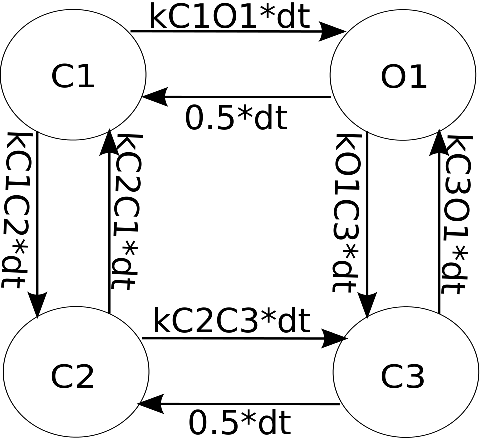
\includegraphics[scale=0.5]{figs/state.pdf}
\caption{The eight possible transitions between four states of a RyR, where the labels on the arrows indicate the
probabilities of the transitions.}
\label{ryrstates}
\end{figure}

在每个细胞里,有约$10000$个钙离子释放单元也叫dyads,这些钙离子释放单元按照$100\times 10\times 10$的三维网格进行排列。每个dyad包含五个不同的小单元,钙离子会在这些小单元里停留,详细的公式和参数可以参考文献\upcite{gaur2011multiscale}。每个dyad空间里,包含15个L-型钙离子通道和$100$个RyRs,它们是随机地活动的。在任何时刻,每个RyR会处于四个状态中的一个,这四个状态用C1、~C2、~C3以及~O1表示。图\ref{ryrstates}中给出了各个状态间可能的转换关系,以及状态间转换的概率,图\ref{ryrstates}状态转换的概率参数是与每个RyR内的钙离子浓度相关的,除了其中从~O1到~C1以及从~C3到~C2的转换概率为常数。处于打开状态(即处于~O1状态)的RyR的个数直接影响到钙离子的流量,进而影响每个细胞内的电压。

dyad中的钙离子浓度可以通过公式\ref{eq:1}至公式\ref{eq:10}来求解。

{
\allowdisplaybreaks
 \begin{eqnarray}
  ca_{\mathrm{ds}}& = & (J_{\mathrm{rel}} + J_{\mathrm{lca}} + ca_{\mathrm{ss}} / \tau_{\mathrm{efflux}})\times \tau_{\mathrm{efflux}}\label{eq:1}\\
  \frac{d\, ca_{\mathrm{ss}}}{dt}& = & \overline{B_{\mathrm{ss}}}\left(  J_{\mathrm{NCX}} + J_{\mathrm{diff\_myo\_ss}} + J_{\mathrm{diff\_ds\_ss}}\right) \label{eq:2}\\
  \frac{d\,ca_{\mathrm{JSR}}}{dt}& = & \overline{B_{\mathrm{JSR}}}\left(J_{\mathrm{rel}} + J_{\mathrm{diff\_NSR\_JSR}}\right) \label{eq:3}\\
  \frac{d\,ca_{\mathrm{NSR}}}{dt}& = & J_{\mathrm{up}} - J_{\mathrm{leak}} - J_{\mathrm{diff\_NSR\_JSR}}  \label{eq:4}\\ 
  \frac{d\,ca_{\mathrm{myo}}}{dt}& = & \overline{B_{\mathrm{myo}}}\left(J_{\mathrm{cab}} + J_{\mathrm{pca}} + J_{\mathrm{NCX}} - J_{\mathrm{up}} + J_{\mathrm{leak}} - J_{\mathrm{diff\_myo\_ss}}\right) \label{eq:5}\\
  Ca_{\mathrm{ds}}& = & (J_{\mathrm{rel}} + J_{\mathrm{lca}} + Ca_{\mathrm{ss}} / \tau_{\mathrm{efflux}})\times \tau_{\mathrm{efflux}}\label{eq:6}\\  
  \frac{\partial Ca_{\mathrm{ss}}}{\partial t}& = & \overline{B_{\mathrm{ss}}} \left(J_{\mathrm{NCX}} + J_{\mathrm{diff\_myo\_ss}} + J_{\mathrm{diff\_ds\_ss}}
+ D_{Ca}\nabla^2Ca_{\mathrm{ss}}\right) \label{eq:7}\\
  \frac{d\,Ca_{\mathrm{JSR}}}{dt}& = & \overline{B_{\mathrm{JSR}}}\left(J_{\mathrm{rel}} + J_{\mathrm{diff\_NSR\_JSR}}\right) \label{eq:8}\\
  \frac{\partial Ca_{\mathrm{NSR}}}{\partial t}& = & J_{\mathrm{up}} - J_{\mathrm{leak}} - J_{\mathrm{diff\_NSR\_JSR}}  +  D_{\mathrm{SR}}\nabla^2 Ca_{\mathrm{NSR}}\label{eq:9}\\					
  \frac{\partial Ca_{\mathrm{myo}}}{\partial t}& = &
                                                     \overline{B_\mathrm{myo}}\left(J_\mathrm{cab} + J_\mathrm{pca} + J_\mathrm{NCX} - J_\mathrm{up} + J_\mathrm{leak} - J_\mathrm{diff\_myo\_ss}\right.\nonumber\\
&&+ \left. D_{Ca}\nabla^2Ca_{\mathrm{myo}}\right)
\label{eq:10}
  \end{eqnarray}
}
%
%\noindent

公式中,$J_{\mathrm{rel}}$是从RyRs到dyad单元间的钙离子流通量,$J_{\mathrm{lca}}$是从L-型钙离子通道到dyad间的钙离子流通量,$\tau_{\mathrm{efflux}}$是dyad空间和膜下空间之间的扩散系数,$J_{\mathrm{NCX}}$是钠离子和钙离子交换在膜下空间产生的电流通量,$J_{\mathrm{diff\_myo\_ss}}$是肌质与膜下空间之间的扩撒流通量,$J_{\mathrm{diff\_ds\_ss}}$是dyad与膜下空间之间的扩撒流通量。$J_{\mathrm{diff\_NSR\_JSR}}$是NSR和JSR间的扩撒流通量,SR泵可以将钙离子从NSR抽到SR中,产生的流通量用$J_{\mathrm{leak}}$来表示。$J_{\mathrm{pca}}$是流过胞质膜的钙离子流通量,膜下空间会被SR和SL瞬间缓冲,瞬间缓冲系数是通过$\overline{B_{\mathrm{ss}}}$来表示的。$\overline{B_{\mathrm{JSR}}}$是CSQN到JSR间的瞬间缓冲系数,$\overline{B_{\mathrm{myo}}}$是从CMDN和TRPN到胞质膜的瞬间缓冲系数。更加详细的关于各个参数和变量的信息可以参考文献\upcite{gaur2011multiscale}。

\subsection{数值策略}
本课题采用随机的方法对L-型钙离子通道和RyRs进行随机模拟,详细的介绍将在\ref{cellImp}中介绍。显式时间积分法被用来求解所有的微分方程(\ref{tissuevoltage})-(\ref{eq:10})。涉及的扩撒项采用中心有限差分的方法进行离散化。而对于单域方程(\ref{tissuevoltage}),使用的是算子分裂方法\upcite{qu1999advanced}。这意味着扩撒项与离子产生的电流项$I_\mathrm{ion}$是分开处理的,后者是通过求解Ord模型中的所有常微分方程得到所有的离子电流,并将所有的离子电流累加起来而得到。

所有的计算流程是发生在一个时间循环内,循环中是每个时间步需要完成的工作,具体包括对所有细胞内的模拟,然后是根据公式\ref{tissuevoltage}对细胞间电压扩撒过程进行计算。每个细胞内的计算包括对所有的dyads进行计算,然后对dyad间的扩撒过程进行计算。具体过程如表\ref{overview}中的伪代码所示,对其中的计算进行高效实现变得非常重要。

\begin{table}
\caption{3D组织模拟计算的伪代码实现}
\label{overview}
\begin{lstlisting}[language=C++, basicstyle=\ttfamily\footnotesize]
Global initialization
  for (int t = 0; t < time steps; t++) {	
    for (int k = 1; k <= cells; k++) {
      Cell computation
      for (int j = 1; j <= dyads; j++) {
        L-type probability calculation
        L-type opening	
        RyR probability calculation
        RyR opening
        Ca concentration computation }
      Dyad diffusion }
    Cell difusion }
\end{lstlisting}
\end{table}


\section{基于多核CPU系统的心脏组织3D模拟的实现}

 \subsection{多级并行}
 
 \subsection{单个细胞内的数值计算实现}
 \label{cellImp}
 



\section{实验结果与分析}
\subsection{实验设置}

\subsection{性能优化实验}

\subsection{扩展性实验}

\subsection{细胞内离子活动实验}

\subsection{心脏组织内异常活动模拟}

\section{小结}



















\chapter{基于大规模异构集群系统的心脏组织模拟的并行优化}
\label{chapbmvc1}

\section{引言}




\section{相关研究}
\subsection{心脏组织模拟的数学模型}



\subsection{心脏组织模拟的并行实现}


\section{心脏组织模拟的数学建模}


\section{心脏组织模拟的高性能并行实现}

 \subsection{心脏组织模拟的tissue-级并行}
 
 \subsection{心脏组织模拟的cell-级并行}

\subsection{心脏组织模拟的dyad-级并行}

\subsection{心脏组织模拟中随机数生成}



\section{实验结果与分析}
\subsection{实验设置}

\subsubsection{心脏组织模拟单设备性能}

\subsection{心脏组织模拟的单节点性能}

\subsection{心脏组织模拟的多节点性能}

\section{小结}
